Os principais problemas do desenvolvimento de software estão associados a Engenharia de Requisitos. Requisitos que não refletem as reais necessidades dos usuários, que sejam incompletos ou inconsistentes, mudanças em requisitos já acordados e dificuldade em chegar em um entendimento comum entre usuários e desenvolvedores são grandes dificuldades relatadas, provocando retrabalho, atrasos no cronograma, custos ultrapassados e insatisfação dos clientes e usuários de software (13).

Tendo em vista a grande importância do Processo de Engenharia de Requisitos, foram criadas ferramentas para a gerência de requisitos, visando apoiar os responsáveis pelo desenvolvimento de software. Características importantes na escolha da ferramenta adequada ao projeto estão relacionadas à capacidade de  armazenar, manter e gerenciar mudanças dos requisitos, além de permitir a rastreabilidade entre requisitos funcionais, casos de testes, cronogramas e código fonte.


\section {Análise de Ferramenta de Gestão de Requisitos}

\subsection{Ferramentas}

Para o presente projeto foram analisadas três ferramentas, afim de escolher dentre elas a que melhor se adaptasse ao contexto e necessidades do mesmo:

1- CodeBeamer

O CodeBeamer é uma plataforma integrada que oferece um conjunto de recursos de Gerenciamento de Requisitos, Desenvolvimento, Teste, Qualidade e outros. A ferramenta fornece escalabilidade Agile, completo gerenciamento de mudança e controle de processo robusto. Possui suporte ao fluxo de trabalho avançado com recursos de colaboração que apoiam metodologias Ágeis, Cascata e Híbridas, além de Gerenciamento de Ciclo de Vida de Aplicativos SAFe. O CodeBeamer permite o gerenciamento dos requisitos para várias variantes do produto de forma colaborativa em todo o ciclo de vida, buscando consistência e conformidade de forma a garantir que o produto atenda às necessidades das partes interessadas.

\FloatBarrier
\begin{figure}[!htpd]
		\centering
		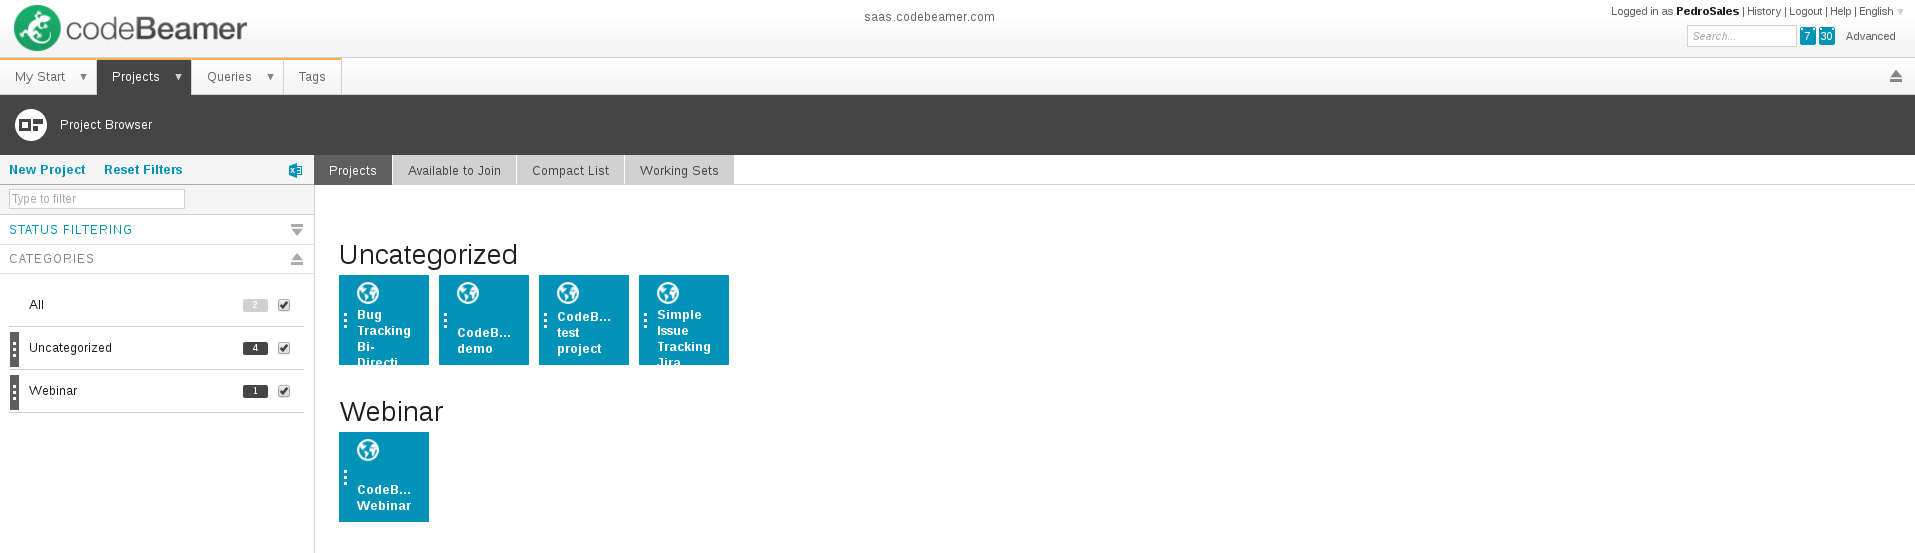
\includegraphics[scale=0.27]{figuras/Code}
		\label{img:SAF}
		\caption{CodeBeamer 1}
\end{figure}
\FloatBarrier


\FloatBarrier
\begin{figure}[!htpd]
		\centering
		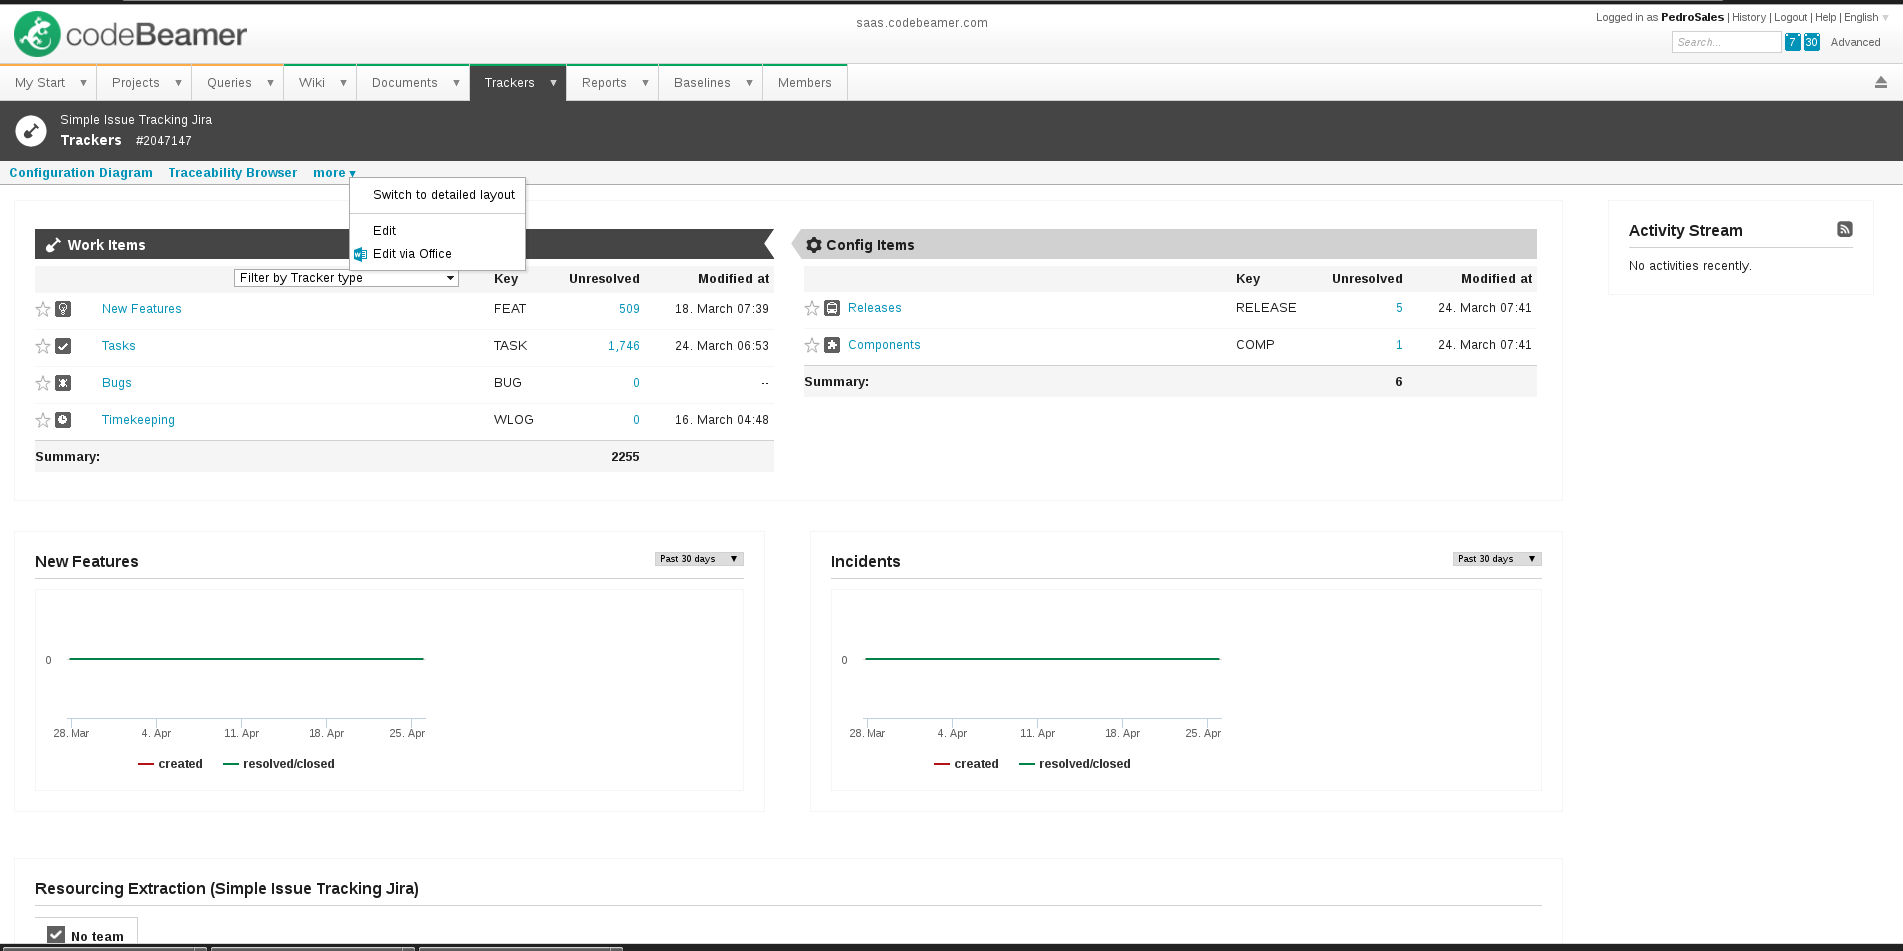
\includegraphics[scale=0.27]{figuras/Code01}
		\label{img:SAF}
		\caption{CodeBeamer 2}
\end{figure}
\FloatBarrier


\FloatBarrier
\begin{figure}[!htpd]
		\centering
		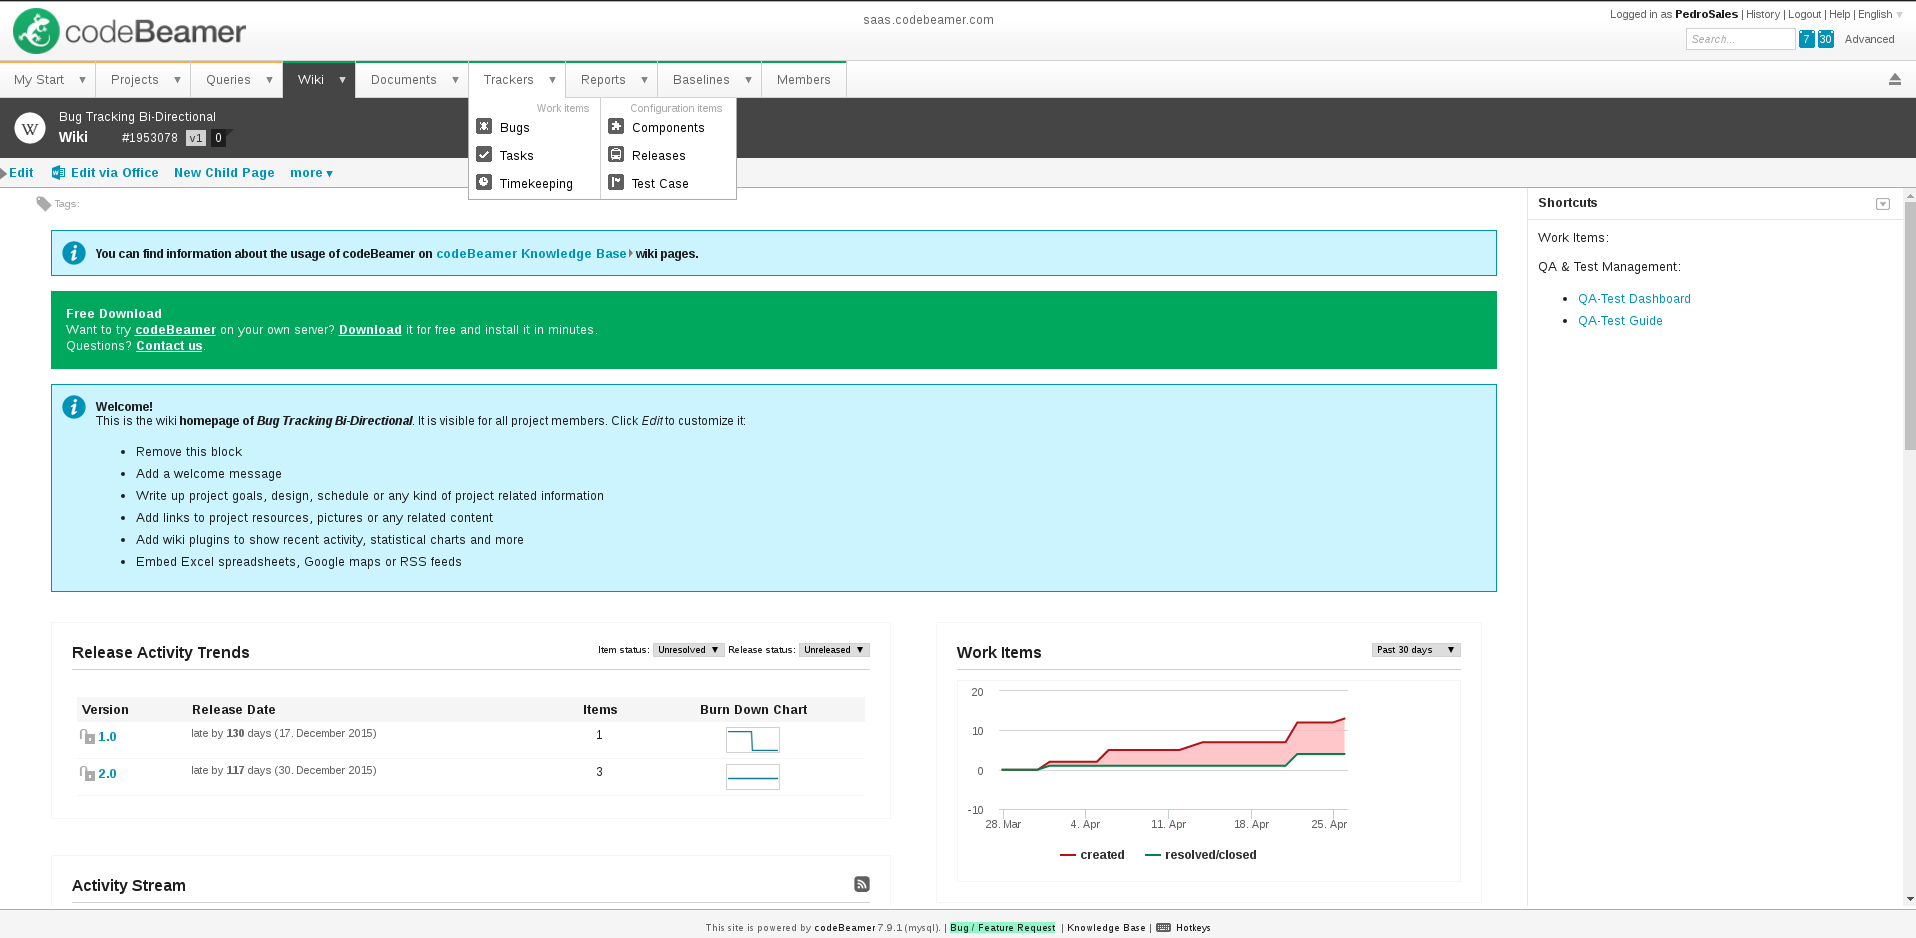
\includegraphics[scale=0.2]{figuras/Code02}
		\label{img:SAF}
		\caption{CodeBeamer 3}
\end{figure}
\FloatBarrier

2- Caliber

O Caliber vem com a proposta de integrar o setor de TI, e o setor de tomadas de decisões, visando assim eliminar as lacunas presentes entre esses dois setores. Uma das grandes vantagens dessa ferramenta é a parte visual, por ser o primeiro produto corporativo a integrar a definição de requisitos com uma ferramenta visual. O Caliber permite a especificação visual dos requisitos funcionais, a execução de quadros gráficos, modelar casos de utilização, e também de cenários, além disso, a ferramenta gera automaticamente exemplos de teste, para comprovar a qualidade do ciclo de vida do software.


\FloatBarrier
\begin{figure}[!htpd]
		\centering
		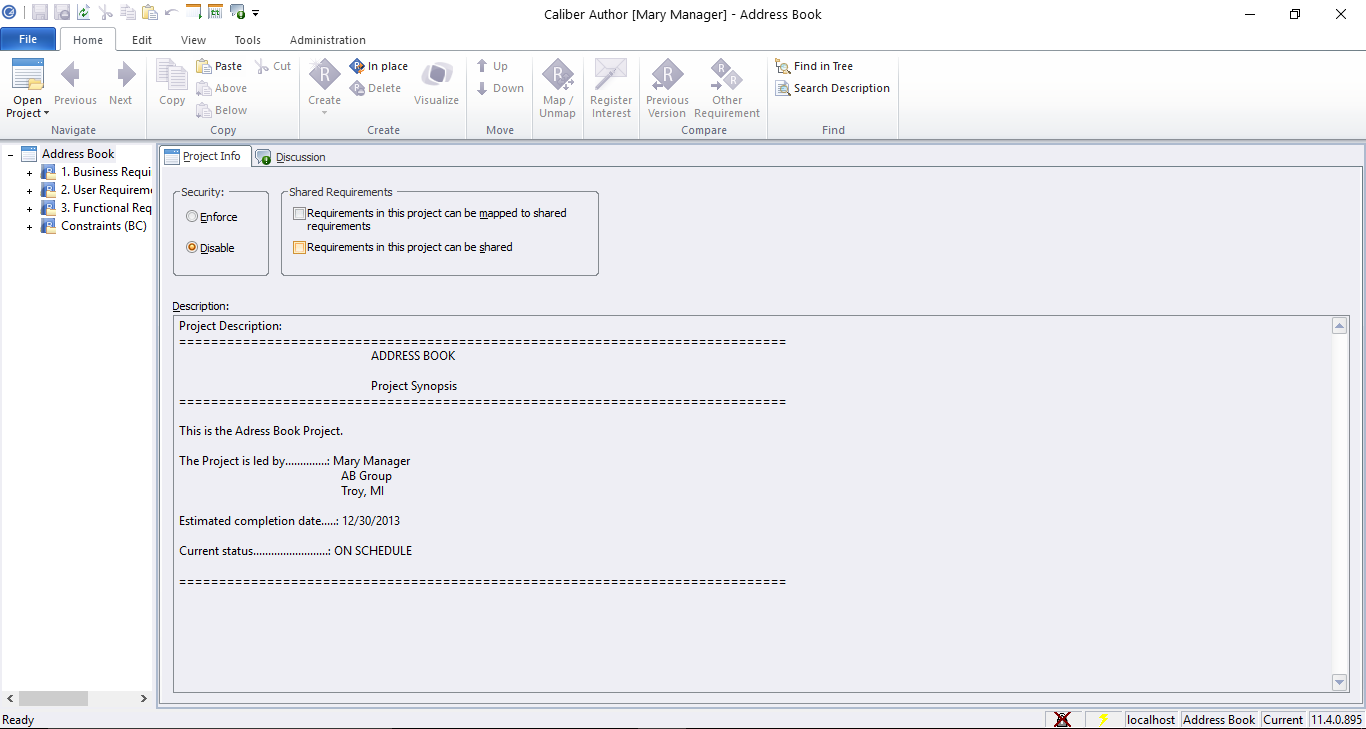
\includegraphics[scale=0.4]{figuras/caliber_1}
		\label{img:SAF}
		\caption{Caliber 1}
\end{figure}
\FloatBarrier

\FloatBarrier
\begin{figure}[!htpd]
		\centering
		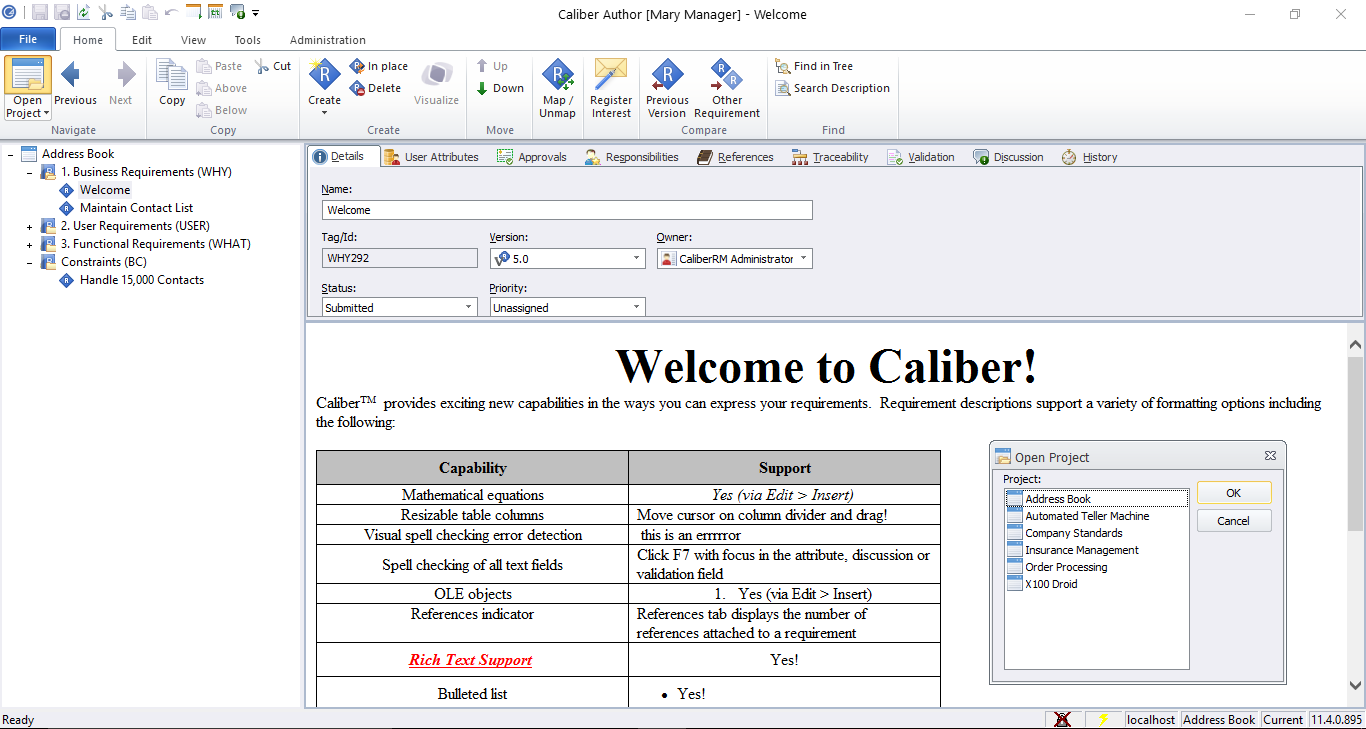
\includegraphics[scale=0.5]{figuras/caliber_2}
		\label{img:SAF}
		\caption{Caliber 2}
\end{figure}
\FloatBarrier

\FloatBarrier
\begin{figure}[!htpd]
		\centering
		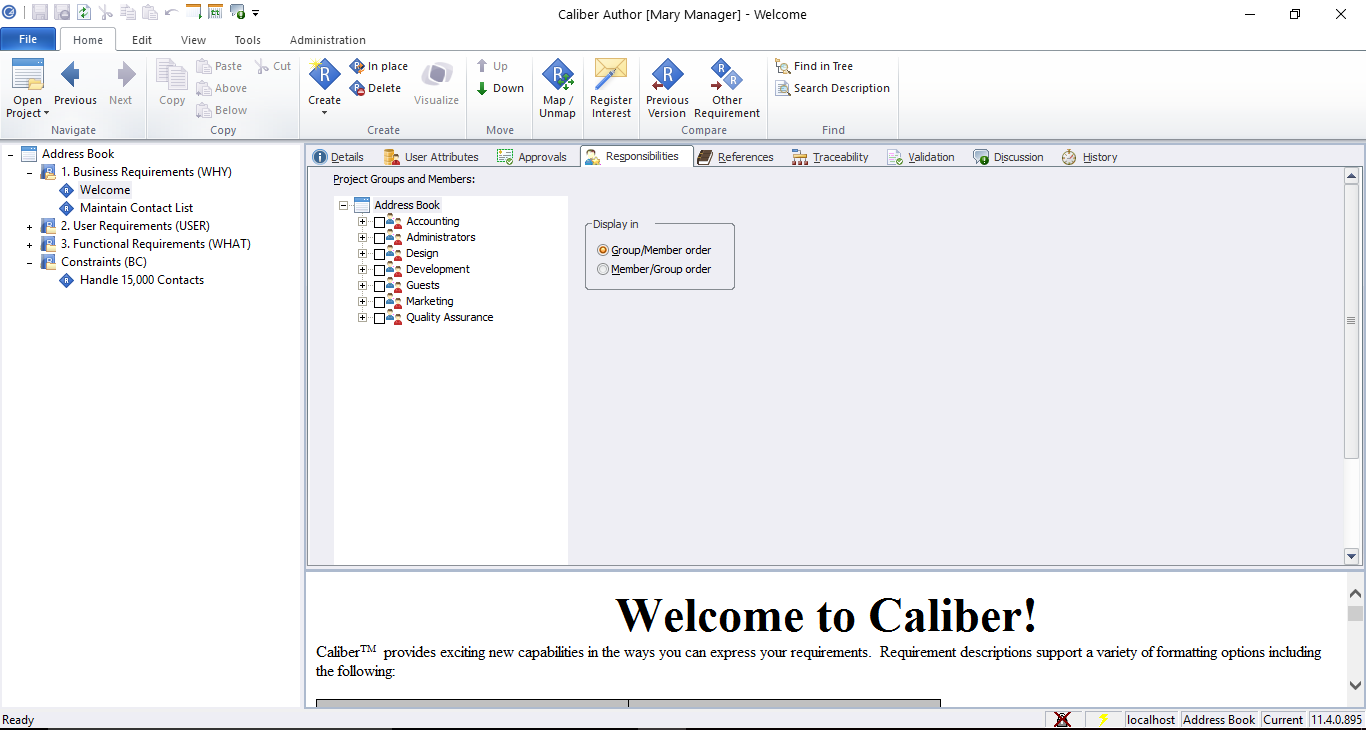
\includegraphics[scale=0.4]{figuras/caliber_3}
		\label{img:SAF}
		\caption{Caliber 3}
\end{figure}
\FloatBarrier


3- Traceloud

TraceCloud é uma solução de Gerenciamento de Requisitos Web, projetada para ser flexível, de forma a poder ser aplicado tanto a metodologias ágeis quanto tradicionais, ser ainda leve e com grande poder de gerenciamento. TraceCloud foi construído em um sistema de Business Intelligence, que identifica e apresenta previamente pontos de conflitos e possui sistema de gerência de falhas, requisitos e testes totalmente integrados. Possui uma grande quantidade de funcionalidades para: bloquear e controlar alterações, compartilhar requisitos, promover a colaboração, integração, fluxo para aprovação de trabalho, rastreabilidade, dinamicidade, documentação dinâmica, controle de versão,  entre outros.

\FloatBarrier
\begin{figure}[!htpd]
		\centering
		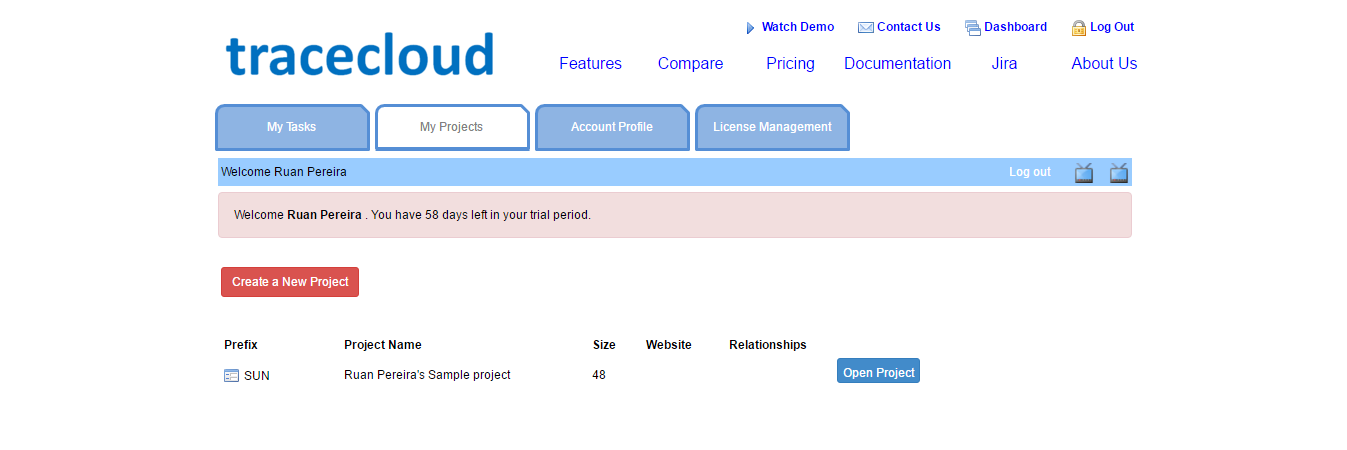
\includegraphics[scale=0.5]{figuras/trace_1}
		\label{img:SAF}
		\caption{Traceloud 1}
\end{figure}
\FloatBarrier

\FloatBarrier
\begin{figure}[!htpd]
		\centering
		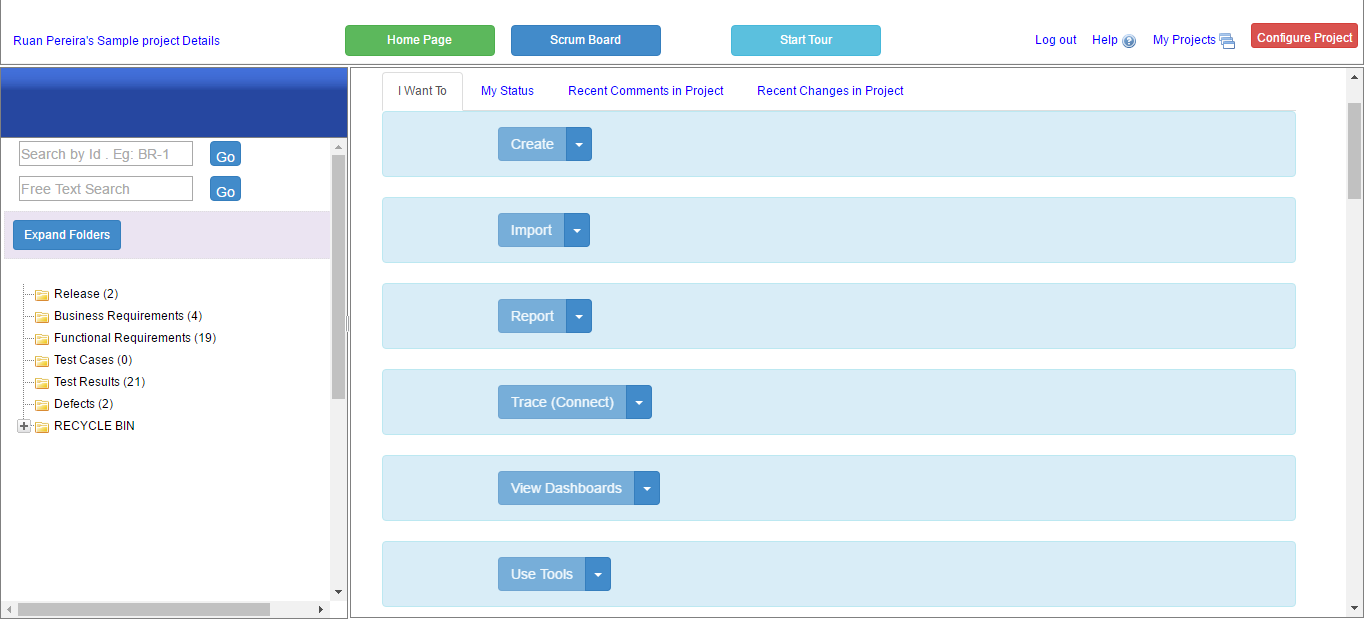
\includegraphics[scale=0.4]{figuras/trace_2}
		\label{img:SAF}
		\caption{Traceloud 2}
\end{figure}
\FloatBarrier

\FloatBarrier
\begin{figure}[!htpd]
		\centering
		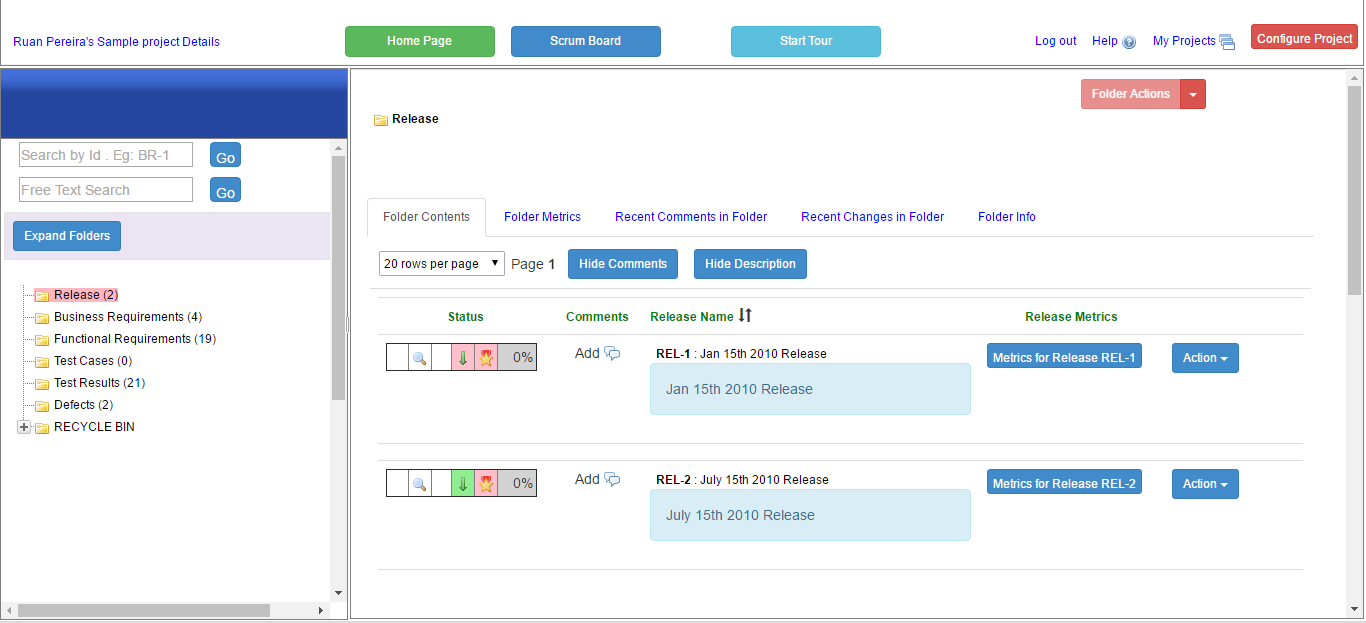
\includegraphics[scale=0.5]{figuras/trace_3}
		\label{img:SAF}
		\caption{Traceloud 3}
\end{figure}
\FloatBarrier



\subsection {Critérios}

Para esta analise, foram listadas as 5 características mais importantes de cada ferramenta para este projeto, referentes à Usabilidade, Rastreabilidade, Gestão de Mudanças, Flexibilidade e Licença.

Em seguidas pontuadas, de 0 a 5 pontos, de forma que, quanto mais próximo da pontuação 5, maior a importância de tal característica para o contexto do projeto, e, consequentemente, a proximidade da pontuação 0 representa o quanto a característica foge do objetivo principal e necessidades para uso da ferramenta neste. Em relação ao critério Licença, a mesma será descrita em relação à ferramenta em enfoque.

\subsection {Descrição dos Critérios}

\begin{table}[\htp]
\centering
\caption{Critérios}
\label{my-label}
\begin{tabular}{|l|l|}
\hline
Critério     & Descrição                                         \\ \hline
Usabilidade &  Evidencia o esforço necessário para utilizar o software por um conjunto de usuários \\ \hline
Rastreabilidade & Eficiência em rastreabilidade bidirecional dos requisitos.\\ \hline
Gestão de Mudanças & O gerenciamento de mudanças está relacionado a procedimentos, processos e padrões que são usados para gerenciar mudanças nos requisitos do sistema (19).\\ \hline
Flexibilidade e Compatibilidade
 & Compatibilidade entre diferentes SO e configurações. \\ \hline
Licença & Relativo a licença de uso da ferramenta. \\ \hline

\end{tabular}
\end{table}
\subsubsection{Usabilidade}

CodeBeamer - O CodeBeamer tem design simples, favorecendo o entendimento de seus elementos e a navegabilidade, tanto na versão desktop quanto web. A ferramenta funciona de forma colaborativa e permite a integração com outras ferramentas, como MS World e Excel, Matlab, Jira, JUnit, Jenkins, entre outros.

Caliber - A solução viabiliza a colaboração, visualização de qualidade, gerenciamento robusto e capacidade de acompanhamento dos requisitos nos planos de fornecimento ágil. Permite a visualização dos requisitos como fluxos de usuários interativos e passíveis de teste para aumentar a clareza e a precisão.

TraceCloud - Tudo relacionado a um requisito, como rastreabilidade, atributos, status de teste, log, informação de versão, status de aprovação e informação básicas estão convenientemente localizado em uma página. Isto reduz a cliques do mouse e torna o sistema mais utilizável. Usa um código de cores para mostrar visualmente requisitos incompletos, que não foram testados ou com problema de rastreabilidade.

\subsubsection{Rastreabilidade}

CodeBeamer - O CodeBeamer garante a rastreabilidade e o gerenciamento de dependências estabelecendo links entre os artefatos. Possui Treceability Browser, uma tabela para mapeamento da rastreabilidade, relacionando dependências rastreadas.

Caliber - O Caliber fornece a geração automática e o relato de tabelas de rastreamento personalizado. O controle integrado detecta imediatamente elementos órfãos e destaca rastros suspeitos, para fornecer uma excelente transparência da qualidade do seu projeto.

TraceCloud - TraceCloud da pleno acesso e controle à instrumentos de rastreabilidade, como TraceMatrix, TraceTrees, Análise de Impacto de Mudanças (CIA), tendo como objetivo ainda a usabilidade, desempenho e escalabilidade.

\subsubsection{Gestão de Mudanças}

CodeBeamer - O CodeBeamer mantém o controle de mudança com um histórico completo de todos os ajustes de requisitos. Fluxos avançados de trabalho permitem personalização do processo, adicionando mecanismos de segurança para garantir que somente pessoas autorizadas façam alterações nos requisitos.

Caliber - O Caliber aposta em uma maior integração entre os requisitos de definição e gestão dos projetos para desenvolvimento de software, de forma a diminuir o tempo de resposta às mudanças de requisitos. O Caliber não possui mecanismo específico para gerência de mudanças de requisitos.

TraceCloud - O TraceCloud possui um sistema para análise de níveis de rastreabilidade para mudanças de requisitos. Também é possível fazer definições de papéis para controle e permissões de modificação de acordo com funções atribuídas aos membros da equipe.

\subsubsection{Flexibilidade e Compatibilidade}

CodeBeamer - CodeBeamer fornece versões desktop para Windows, Mac e Linux, além da versão em camada SaaS. Conta com aplicativos customizados, integração com pacote Office, softwares de Design, Modelagem, Gerenciamento de Defeitos, entre outros.

Caliber - Suportado somente em Windows 7, Windows 8/8.1, Windows Vista e Windows XP. Possui integração com outros plug-ins da Micro Focus, além de integração com Microsoft Visual Studio e Eclipse.

TraceCloud - Aplicação em camada SaaS. Possui integração com pacote Office (Word e Excel) e faz integração com projetos já existentes via serviço RESTFul Web API (JASON).

\subsubsection{Licença}

CodeBeamer - Possui versão trial de avaliação de 30 dias, havendo alternativas de licença anual ou vitalícia do produto, que variam de 1080 a 3240 euros para anual e 1800 a 5400 euros para vitalício.

Caliber - Possui versão de avaliação de 30 dias. Não foram encontradas informações para valores de contratação.

TraceCloud - Possui versão gratuita por tempo limitado. Para as versões pagas existem as licenças para usuário: leitura e estrita, com criação ilimitada de projetos e requisitos por 30 dólares por mês; somente leitura, com criação ilimitada de projetos e requisitos por 25 dólares por mês. Existe também a licença para projeto: 350 dólares por mês para projetos com menos de 5000 requisitos, 700 dólares para projetos entre 5000 e 10000 requisitos e 1000 dólares por mês para projetos com mais de 10000 requisitos.

\subsection{Pontuação dos Critérios}

\begin{table}[\htp]
\centering
\caption{Pontuação ferramentas}
\label{my-label}
\begin{tabular}{llll}
 & CodeBeamer & Caliber & Traceloud \\
Usabilidade & 3 & 4 & 5 \\
Rastreabilidade & 5 & 5 & 5 \\
Gestão de Mudanças & 5 & 2 & 4 \\
Flexibilidade e Compatibilidade & 5 & 3 & 4 \\
Licença & 3 & 3 & 4 \\
Total & 21 & 17 & 22
\end{tabular}
\end{table}


\subsection{Ferramenta Escolhida}

Tomando por base os critérios descritos no tópico Descrição dos Critérios (8.1.3) e a pontuação atribuída pelo grupo a cada uma das ferramentas (Pontuação dos Critérios - 8.1.4), pode-se concluir que a ferramenta TraceCloud apresentou-se como a melhor alternativa dentre as ferramentas consideradas. Isto se dá por obter nota máxima em Usabilidade e Rastreabilidade, que são critérios de extrema importância para o sucesso do projeto, e ainda nota alta em Gestão de Mudanças, que é de grande importância, e em todos os outros critérios, de forma a não apresentar discrepâncias e pontos fracos que possam de alguma forma vir a afetar de forma prejudicial o pleno desenvolvimento do trabalho, impedindo-o de obter sucesso em sua conclusão.
